%\subsection{Signal event definition}
The experimental signature of interest here is identical to the $13\tev$ analysis detailed in Chapter~\ref{ch:ssww13tev}: two prompt leptons (electrons or muons) with the same charge, missing transverse energy, and two jets.
Once again the two leading jets are required to have a large angular separation and a high combined invariant mass to enhance the EWK VBS production.


\subsection{Sensitivity to longitudinal polarization}\label{sec:sswwupgrade_longitudinal_sens}

\begin{figure}[htp]
  \centering
  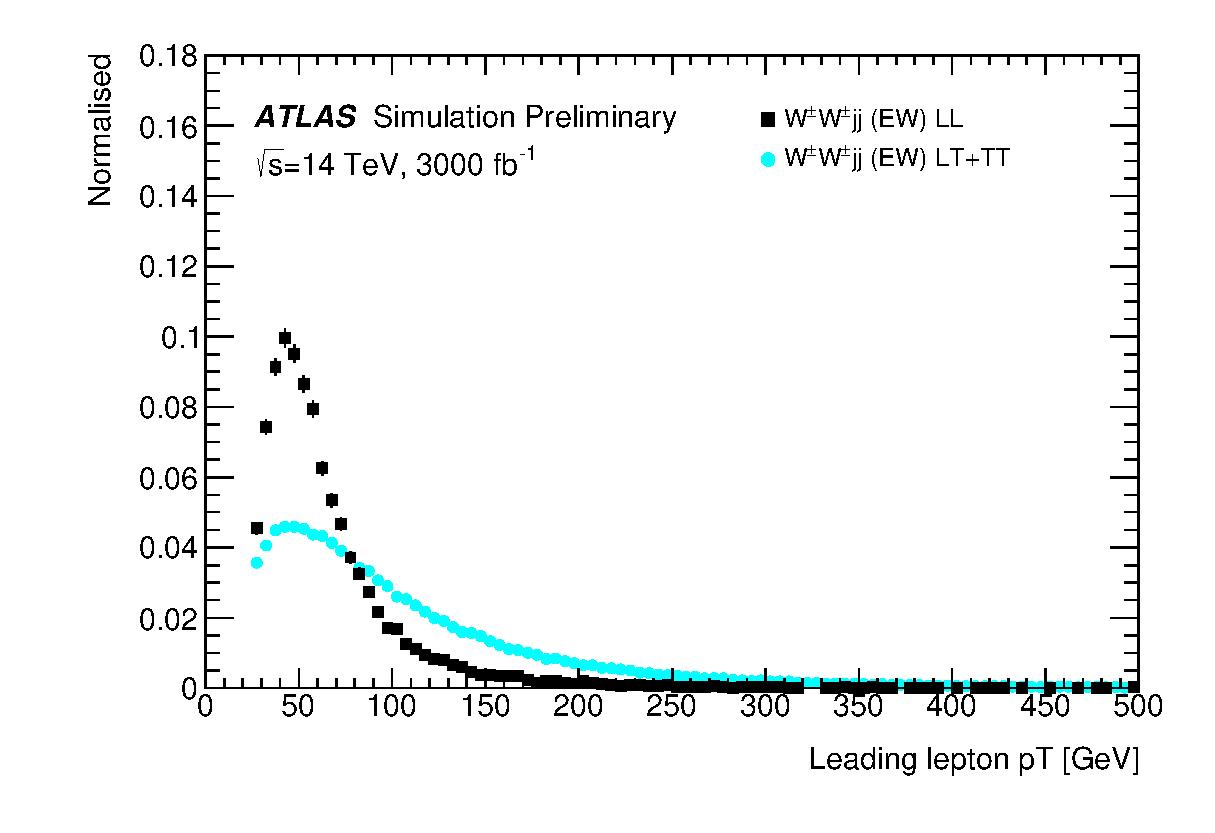
\includegraphics[width=0.8\textwidth]{figs/ssww_upgrade/polarization/lepton0_pt_pass9}\\
  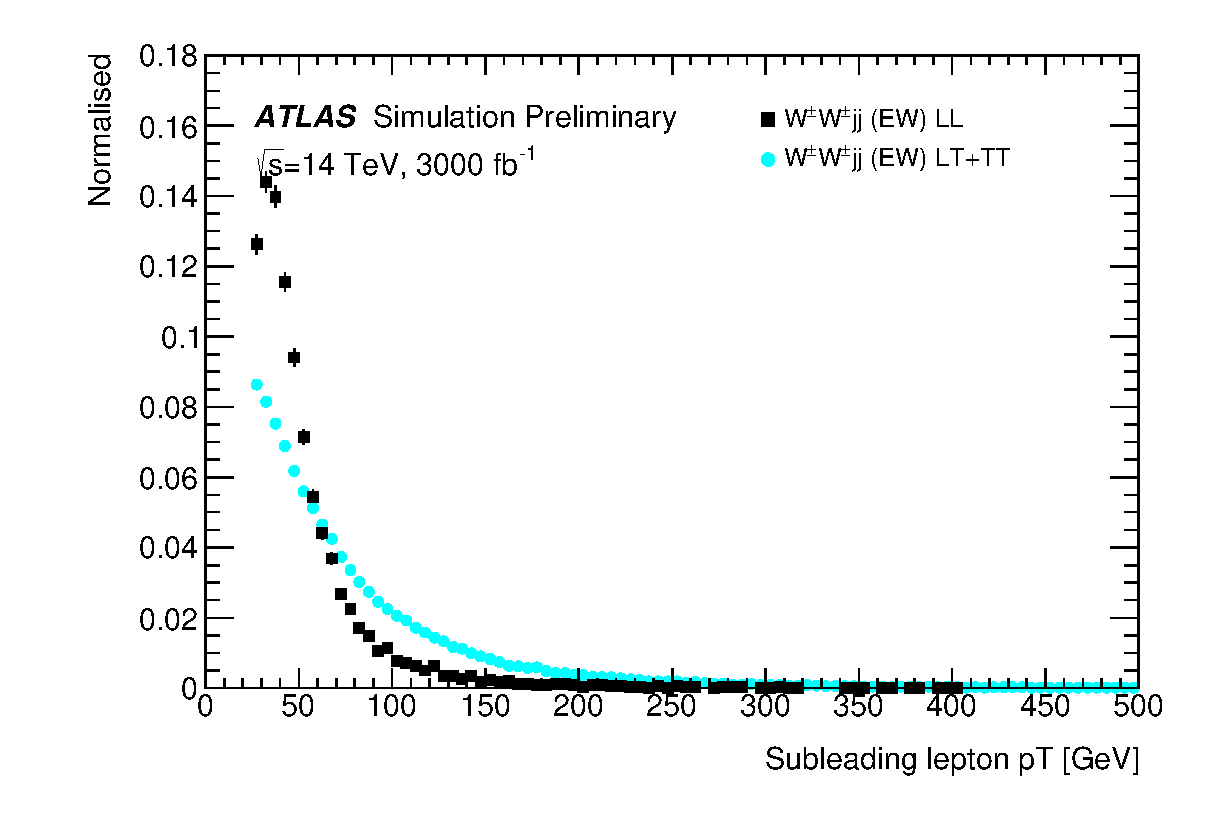
\includegraphics[width=0.8\textwidth]{figs/ssww_upgrade/polarization/lepton1_pt_pass9}
  \caption{Comparison of the leading (top) and subleading (bottom) lepton $\pt$ distributions for purely longitudinal (LL, black) and mixed polarization (LT+TT, cyan) \ssww events.  Plots from \cite{2018.ssww-upgrade-support}.}
  \label{fig:polarization_leppt}
\end{figure}

\begin{figure}[htp]
  \centering
  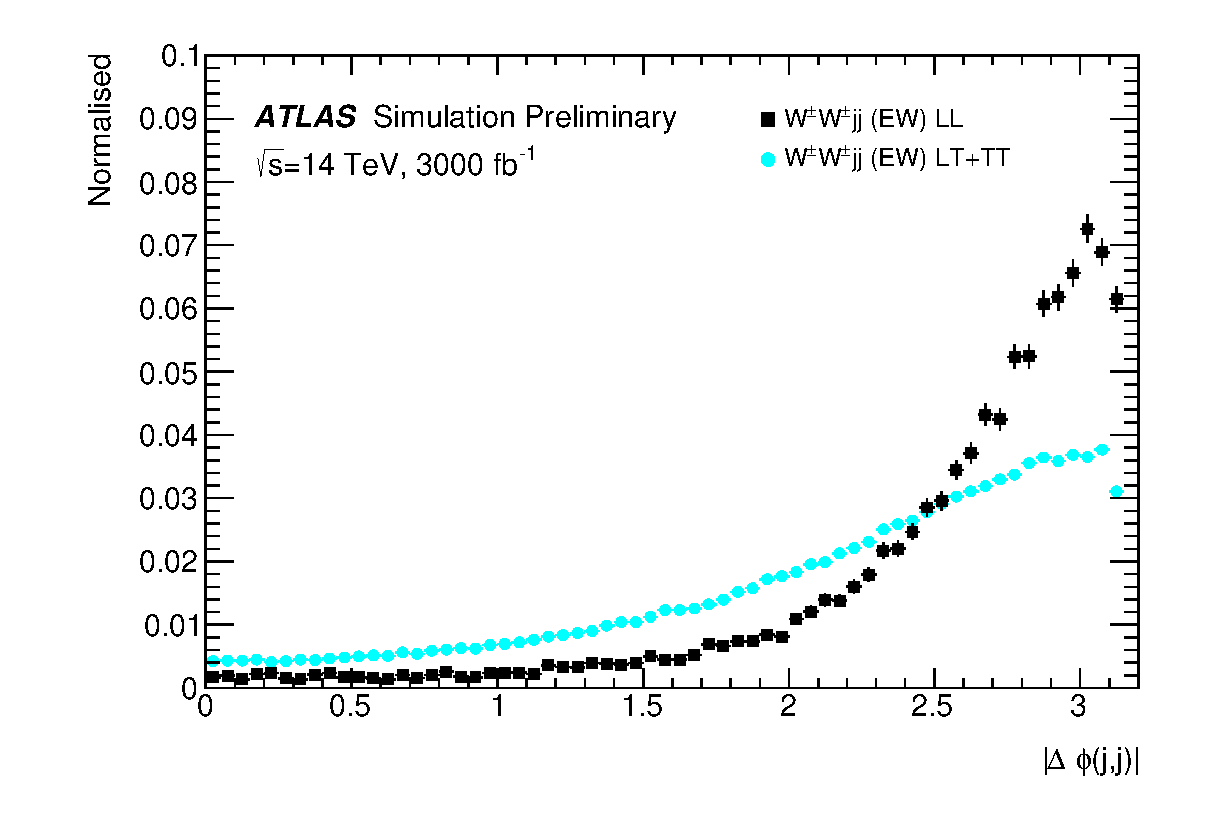
\includegraphics[width=0.8\textwidth]{figs/ssww_upgrade/polarization/dijet_absdphijj_pass9}
  \caption{Comparison of the azimuthal dijet separation ($|\dphijj|$) for purely longitudinal (LL, black) and mixed polarization (LT+TT, cyan) \ssww events.  Plot from \cite{2018.ssww-upgrade-support}.}
  \label{fig:polarization_dphijj}
\end{figure}
